\documentclass[10pt,twocolumn]{article}
\usepackage[a4paper,margin=1.8cm,columnsep=0.55cm]{geometry}
\usepackage{amsmath,amssymb,amsthm}
\usepackage{tabularx,booktabs}
\usepackage{microtype}
\usepackage{tikz}
\usetikzlibrary{positioning,arrows.meta}
\usepackage{fancyhdr}
\setlength{\headheight}{14pt}
\fancypagestyle{preprintfirst}{\fancyhf{}%
  \fancyhead[L]{\small\itshape A Synthesis of the Information Universe preprint -- not peer reviewed}%
  \renewcommand{\headrulewidth}{0pt}\fancyfoot[C]{\thepage}}
\usepackage[hidelinks]{hyperref}
\newcolumntype{Y}{>{\raggedright\arraybackslash}X}

\newtheorem{theorem}{Theorem}
\newtheorem{proposition}{Proposition}
\newtheorem{corollary}{Corollary}
\theoremstyle{definition}
\newtheorem{ansatz}{Ansatz}
\newtheorem{reading}{Reading}
\newcommand{\Thq}{\textsf{[Th\_coqc]}}
\newcommand{\Tone}{\textsf{[Tier-1]}}
\newcommand{\Dr}{\textsf{[Dr]}}
\newcommand{\Ax}{\textsf{[AX/import]}}
\newcommand{\Open}{\textsf{[OPEN]}}
\newcommand{\code}[1]{\texttt{#1}}

\title{\bfseries A Synthesis of the Information Universe:\\
Relativity and Mass as Readouts of Retained Distinctions,\\
Assembled from Classical Equations over a Machine-Checked Kernel}
\author{Yaoharee Lahtee\\[2pt]
\small ORCID: 0009-0005-3861-0626\\
\small Open Civil Science Initiative, Bangkok, Thailand}
\date{\small Synthesis note over kernel state C41--C57 + bridges \;\textbullet\; \today}

\begin{document}
\maketitle
\thispagestyle{preprintfirst}

\begin{abstract}
\noindent
We synthesize an information-first account of relativity and mass from equations whose
owners span Euler and Lagrange to Jacobson, anchored --- joint by
joint --- on a machine-checked kernel of exact rational-arithmetic theorems (Coq~8.18.0,
axiom-free at Tier~0; every \code{Print Assumptions} reported). The kernel establishes,
as theorems: a double stationarity principle in which the field recurrence and the
retention of graph edges are the two first-variation readouts of one quadratic action;
an exact two-way balance between per-edge field strain and an affine function of Forman
curvature; monotone laws of curvature and spectral data under retention; a per-edge
frequency ceiling; the completeness of the lattice edge frame for symmetric two-tensors
with an exact polarization key; an exact inside/outside/cut partition of the quadratic
form of any graph against any region; and a Clausius-form restatement of the retention
balance, $\delta E \le T\,\delta S$, as a two-way implication given a single disclosed
identification. On this base we assemble the mass chain
retention $\to$ degree $\to$ curvature $\to$ internal-frequency ceiling
$\to$ $\tau_c$ $\to$ $m$, with exactly one disclosed identification
($\tau_c = 1/\omega_{\mathrm{int}}$), yielding a curvature-limited mass bound
$m \le (\hbar/2c^2)\sqrt{(2K/M)(4-F_{\min})}$ whose contrapositive states that
sufficiently large mass \emph{forces} negative combinatorial curvature. We then read
special and general relativity as the economics of retained distinctions ---
no universal reader, congestion of local update budgets, geometry as ledger --- and
mass as a distinction addressed to itself. To our knowledge, no other discrete-gravity programme --- causal sets, Regge
calculus, or hypergraph dynamics --- possesses a machine-checked kernel of any size;
here the entire supporting chain is one. Interpretive claims are tagged and separated
from theorems throughout; the axiomatic basis is stated explicitly, the assembly is
audited for circularity, and the open remainder is enumerated by name. Nothing in this
note claims a derivation of the Einstein field equations; what is claimed is a
theorem-anchored precursor with every non-theorem joint disclosed.
\end{abstract}

\noindent\textbf{Keywords:} retained distinction; machine-checked proof (Coq);
discrete gravity; Forman curvature; spectral ceiling; mass; holographic screen;
Clausius relation; Jacobson thermodynamics; tensor frame; reproducibility.

\paragraph*{Preprint notice.} This manuscript is a preprint and has not yet
undergone formal peer review. Every machine-checked claim is nonetheless
independently confirmable by recompiling the delivered Coq sources
(Table~\ref{tab:artifacts}, pinned by commit and hash prefix); interpretive
readings, disclosed ansatz, and the programme postulate remain provisional until
independently reviewed.

\section{Introduction and claim discipline}\label{sec:intro}

The title's claim is meant literally and narrowly: a \emph{synthesis} here is an
assembly in which every constituent equation is classical and owned (the ownership
ledger of Section~\ref{sec:open}), the substrate --- retained distinctions,
$\delta_R$ --- and the welds are the programme's, and every joint carries an audited
tag. Nothing more cosmic is claimed by the word ``universe'' than the closed loop the
note actually exhibits: distinction $\to$ retention $\to$ geometry $\to$ mass
$\to$ back to the pricing of distinctions. The assembly obeys the programme's
razor throughout: the continuum, and physics stated in it, enter only as
\emph{readouts} of the discrete substrate, never as its root.

This note assembles three strands developed in the URCF/PGFT programme --- the mass
chain, the tensor content of per-edge strain, and the holographic (Clausius) form of
the retention balance --- into a single account of what relativity and mass \emph{are}
when read from an information-first substrate. The account has an unusual epistemic
shape, which we state before any physics.

Every claim in this note carries one of five tags. \Thq{} marks statements that are
theorems of a Coq~8.18.0 kernel over exact rationals, compiled with exit status~0 and
\emph{Closed under the global context} at every \code{Print Assumptions}; the artifact
inventory is Table~\ref{tab:artifacts}. \Tone{} marks readout-limit statements whose
axiom profile is exactly \code{sig\_forall\_dec} plus functional extensionality (no
\code{classic}). \Ax{} marks disclosed identifications or imported results, cited at
their own tier. \Dr{} marks interpretive readings: they are anchored on theorems but
are not themselves theorems. \Open{} marks the enumerated remainder.

\paragraph{Axiomatic basis, explicitly.} The full foundation of this note is:
\emph{(i)}~the Tier-0 kernel, which uses \textbf{no axioms whatsoever} --- every
theorem closes under the global context of Coq's logic alone;
\emph{(ii)}~two Tier-1 readout files, using exactly \code{sig\_forall\_dec} and
functional extensionality, and nothing classical;
\emph{(iii)}~a definitional layer (Forman $F$, the functionals $S_{\mathrm{geo}}$,
$S_{\mathrm{count}}$, the frame) --- definitions, not assumptions;
\emph{(iv)}~three disclosed identifications (Ansatz~C, H, T), mutually independent,
none of which feeds back into any kernel theorem;
\emph{(v)}~two imports at literature tier: Jacobson's argument and the PGFT mass
relation $m=\hbar/(2\tau_c c^2)$, the latter carrying $\hbar$ and $c$ as imported
constants; and \emph{(vi)}~free parameters $\alpha,\beta,K,M,s_0$, fixed only at
the \Dr{} dictionary. Everything below rests on (i)--(vi) and nothing else.

\paragraph{Contributions.} Against that basis, the note's claims to novelty are
four, stated offensively here and defended in Sections~\ref{sec:circ}--\ref{sec:open}:
\emph{(C1)}~the epistemic standard --- nineteen Tier-0 files, $151$ kernel-closed
checks: to our knowledge the first machine-checked kernel in any discrete-gravity
programme, where competing programmes argue in prose (machine-checked
\emph{continuum} relativity does exist --- axiomatic Minkowski spacetime in
Isabelle/HOL \cite{schutzformal,stannett} --- and is complementary rather than
prior: those works formalize the classical theory's axioms, and mechanized numerical
analysis has verified continuum wave schemes \cite{boldo}, not a discrete substrate
with its own dynamics);
\emph{(C2)}~the tier-factored assembly itself, with an acyclic dependency structure
audited in Section~\ref{sec:circ} --- a way of being sweeping and honest at once;
\emph{(C3)}~the welds, none found in prior literature: the retention balance pricing
a tensor evaluation (two-way), the dissipation threshold pair as a native, checkable
horizon, the curvature-monotone mass cap with its contrapositive (mass \emph{forces}
curvature), the cosmological term as the structurally forced affine part of any
benefit function, and the rigidity result that one global lens forces a non-constant,
curvature-dependent temperature;
\emph{(C4)}~the two-arm architecture: mass and holography arrive at the
precursor's two sides --- source content and equation form --- independently, sharing
no ansatz, so the failure of either identification leaves the other standing.

The discipline matters because the note's central move --- ``mass is a retained
distinction addressed to itself'' --- is a \Dr{} sentence. What distinguishes it from
free-floating metaphor is that every load-bearing clause beneath it resolves to a named
theorem with a SHA-256 hash, and every clause that does not is listed in
Section~\ref{sec:open}. The reader is invited to audit rather than believe.

\section{Literature: the classical stream and the modern tiers}\label{sec:lit}

The synthesis draws on, and must be positioned against, ten streams. We review
them with their owners; each paragraph closes with where the present programme
stands relative to it. Table~\ref{tab:streams} condenses the positioning;
Figure~\ref{fig:dag} draws the assembly itself.

\begin{table*}[t]
\centering\footnotesize
\begin{tabularx}{\textwidth}{@{}lYYY@{}}
\toprule
Stream & Representative owners & Establishes & This note adds\\
\midrule
Relativity foundations & Minkowski; Robb; Zeeman; Schutz & geometry from causal order & order-first, mechanized on graphs (C45) \Thq\\
Discrete spacetime & Regge; Bombelli et al.; Loll; Rovelli--Smolin; Wolfram & substrate ontologies & a machine-checked kernel; the retention balance \Thq\\
Thermodynamic gravity & Bekenstein; Hawking; Unruh; Jacobson & horizons are thermal; Einstein as state equation & Clausius form as iff; native horizon pair \Thq{}+\Ax\\
Holography \& entanglement & 't~Hooft; Susskind; Maldacena; RT; Van~Raamsdonk & area laws; geometry from entanglement & exact cut partition; rank-limited coupling \Thq\\
Emergent gravity & Sakharov; analogue gravity; Weinberg--Witten & precedents; the graviton constraint & precursor-level claims; constraint recorded \Dr\\
Information physics & Shannon; Szil\'ard; Landauer; Wheeler & the bit costs energy; it-from-bit & $\delta_R$ as priced pregeometry \Thq{}+\Dr\\
Quantum \& reconstructions & Stinespring--Choi--Kraus; Hardy; CDP & operational structure of QM & \code{kraus\_completeness} at the Tier-0 root \Thq\\
Spectral \& discrete curvature & Fiedler; Chung; Anderson--Morley; Forman; Ollivier & spectra, bounds, curvatures & ceiling composed with retention; the mass cap \Thq{}+\Ax\\
Mass \& internal clock & de~Broglie; Dirac; Schr\"odinger; Hestenes & the clock reading of mass & curvature-capped clock; mass forces curvature \Thq{}+\Ax\\
Variational \& verified computation & Euler--Noether; Marsden--West; Boldo; Gonthier & discrete mechanics; verified schemes & the substrate itself verified, not a scheme \Thq\\
\bottomrule
\end{tabularx}
\caption{The ten streams in one view: what each owns, and the marginal addition
this note claims against it, tagged. Full citations in the text of this section.}
\label{tab:streams}
\end{table*}

\begin{figure*}[t]
\centering
\resizebox{\textwidth}{!}{%
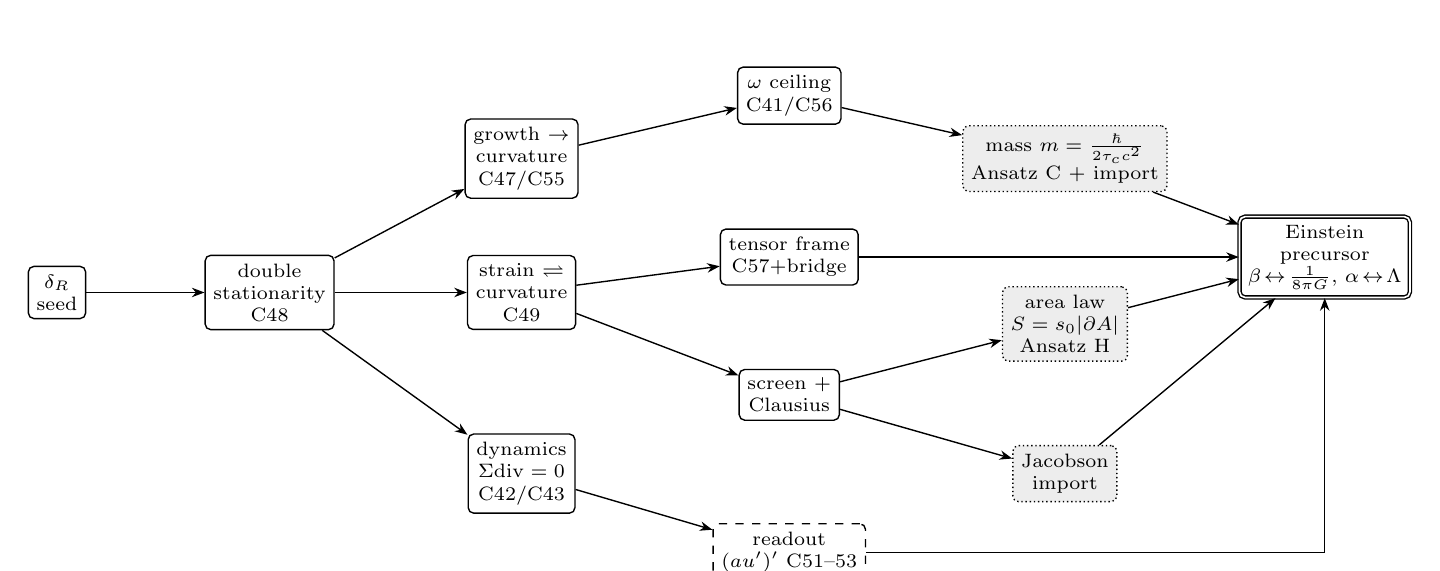
\begin{tikzpicture}[
  every node/.style={draw, rounded corners=2pt, align=center,
    font=\scriptsize, inner sep=3pt, line width=0.5pt},
  th/.style={solid},
  tone/.style={dashed},
  ans/.style={fill=gray!14, densely dotted},
  tgt/.style={double, double distance=0.6pt},
  e/.style={-{Stealth[length=1.6mm]}, line width=0.5pt}]
\node[th]  (S)  at (0,0.4)     {$\delta_R$\\seed};
\node[th]  (DS) at (2.7,0.4)   {double\\stationarity\\C48};
\node[th]  (GC) at (5.9,2.1)   {growth $\to$\\curvature\\C47/C55};
\node[th]  (CB) at (5.9,0.4)   {strain $\rightleftharpoons$\\curvature\\C49};
\node[th]  (DY) at (5.9,-1.9)  {dynamics\\$\Sigma\mathrm{div}=0$\\C42/C43};
\node[th]  (CE) at (9.3,2.9)   {$\omega$ ceiling\\C41/C56};
\node[th]  (TF) at (9.3,0.85)  {tensor frame\\C57+bridge};
\node[th]  (SC) at (9.3,-0.9)  {screen +\\Clausius};
\node[tone](RO) at (9.3,-2.9)  {readout\\$(au')'$ C51--53};
\node[ans] (MA) at (12.8,2.1)  {mass $m=\frac{\hbar}{2\tau_c c^2}$\\Ansatz C + import};
\node[ans] (AL) at (12.8,0)    {area law\\$S=s_0|\partial A|$\\Ansatz H};
\node[ans] (JA) at (12.8,-1.9) {Jacobson\\import};
\node[tgt] (EI) at (16.1,0.85) {Einstein\\precursor\\$\beta\!\leftrightarrow\!\tfrac{1}{8\pi G}$, $\alpha\!\leftrightarrow\!\Lambda$};
\draw[e] (S) -- (DS);
\draw[e] (DS) -- (GC); \draw[e] (DS) -- (CB); \draw[e] (DS) -- (DY);
\draw[e] (GC) -- (CE); \draw[e] (CB) -- (TF); \draw[e] (CB) -- (SC);
\draw[e] (DY) -- (RO);
\draw[e] (CE) -- (MA); \draw[e] (SC) -- (AL); \draw[e] (SC) -- (JA);
\draw[e] (MA) -- (EI);
\draw[e] (AL) -- (EI);
\draw[e] (JA) -- (EI);
\draw[e] (TF) -- (EI);
\draw[e] (RO.east) -| (EI.south);
\end{tikzpicture}}
\caption{The assembly DAG from seed to precursor. Solid boxes: \Thq{}
(axiom-free); dashed: \Tone{}; gray dotted: disclosed ansatz and imports ---
confined to the single layer before the target; double border: \Dr{} target.
The tensor-frame arm runs level through the gap in the ansatz layer and the
readout arm passes beneath it: both reach the target touching no ansatz. Open remainder, by name:
the readout limit, \textsc{ob-forman-ricci}, and tensor evolution.}
\label{fig:dag}
\end{figure*}

\emph{Foundations of relativity.} Minkowski geometrized simultaneity's failure
\cite{minkowski}; Robb showed already in 1914 that the geometry can be axiomatized
from the causal order alone \cite{robb}, Zeeman proved that causality determines
the Lorentz group \cite{zeeman}, Malament that causal order fixes the topology
\cite{malament}, and Schutz gave the modern independent
axiomatization \cite{schutz97}, recently formalized in Isabelle/HOL
\cite{schutzformal}, with first-order relativity verified in the
N\'emeti school's program \cite{stannett}. \emph{Position:} the kernel's
causal-signature file sits squarely in Robb's order-first lineage --- sign,
cones, and the $(1,3)$ cell recovered from comparability --- mechanized at the
graph level rather than the continuum.

\emph{Discrete and emergent spacetime.} Regge replaced metrics by edge lengths
\cite{regge}; causal sets took partial order as ontology \cite{bombelli}; causal
dynamical triangulations recovered four-dimensionality numerically \cite{cdt};
loop quantum gravity and its spin-network ancestry discretized geometry's operators
\cite{rovellismolin,penrose}; quantum graphity \cite{graphity}, 't~Hooft's cellular
automaton program \cite{thooftca}, and Wolfram's hypergraph rewriting \cite{wolfram} (a book-length programme
rather than a refereed result) evolve the graph itself, as we do. \emph{Position:} the programme
shares the substrate intuition of this stream and differs on standard of evidence:
to our knowledge none of these possesses a machine-checked kernel (C1), and the
retention balance --- geometry selected by the \emph{same} action whose other
variation is the field equation --- appears in none.

\emph{Thermodynamic gravity.} On the classical base of Clausius
\cite{clausius}, Boltzmann \cite{boltzmann}, and Gibbs \cite{gibbs}:
Bekenstein's area entropy \cite{bekenstein},
Hawking's radiation \cite{hawking}, and Unruh's acceleration temperature
\cite{unruh} made horizons thermodynamic; Jacobson inverted the logic ---
Einstein's equation as an equation of state \cite{jacobson} --- with
Padmanabhan's program broadening it \cite{padmanabhan} and Verlinde recasting
gravity as entropic force \cite{verlinde}. \emph{Position:} the note's
holographic arm supplies the \emph{form} of Jacobson's premises as theorems
(screen partition; Clausius form at joint stationarity; the threshold pair as
native horizon) and imports his conclusion, with the two identifications
disclosed as lenses.

\emph{Holography and entanglement.} Dimensional reduction \cite{thooft93} and the
holographic principle \cite{susskind} culminated in AdS/CFT \cite{maldacena};
Bousso bounded entropy covariantly \cite{bousso}; Ryu--Takayanagi tied entanglement
to area \cite{rt}, Van~Raamsdonk read spacetime as built from entanglement
\cite{vanraamsdonk}, and tensor networks gave the geometry a circuit form
\cite{swingle}. The correspondence became computational in \cite{witten98,gkp};
the information paradox \cite{hawking76} and the Page curve \cite{page} made
unitarity the battleground; the first law of entanglement recovered linearized
Einstein equations \cite{faulkner}, Jacobson recast the full equation as
entanglement equilibrium \cite{jacobson2016}, bulk locality was rebuilt as quantum
error correction \cite{adh,happy}, and ER${}={}$EPR conjectured geometry from
entanglement outright \cite{erepr}. \emph{Position:} the exact cut partition is
the classical-strain sibling of this quantum stream --- everything the exterior
learns passes through the cut, and the finite-rank coupling across it is the
strain-level shadow of the error-correcting reading of bulk locality --- while the
quantum layer of URCF is developed elsewhere and no entanglement claim is made
here.

\emph{Emergent gravity and its named constraints.} Sakharov derived gravity as an
induced elasticity of the vacuum \cite{sakharov}; Unruh built sonic horizons
\cite{unruh81}, grown into the analogue-gravity program \cite{blv} and Volovik's
condensed-matter universe \cite{volovik}; Anderson's \emph{more is different}
\cite{anderson72} is the stream's manifesto. Against emergent routes stands Weinberg--Witten \cite{weinbergwitten}, binding
under its stated hypotheses (a Lorentz-covariant conserved stress tensor and
massless particles of spin ${>}1$). \emph{Position:} the note's claims stop
at the precursor and assert no emergent graviton; Weinberg--Witten is recorded
here as a named constraint any completion must face, not an objection deferred.

\emph{Information physics.} Shannon quantified distinction \cite{shannon};
Brillouin bound it to negentropy \cite{brillouin}; Szil\'ard priced it against
work \cite{szilard}; Landauer made erasure thermodynamic \cite{landauer}, with
Bennett's reversibility analysis \cite{bennett} and Jaynes's inference reading of
statistical mechanics \cite{jaynes} completing the classical triangle;
Bekenstein bounded information by area and energy \cite{bekbound}. Zuse
\cite{zuse} and Fredkin \cite{fredkin} proposed the computing universe; Lloyd
counted its operations \cite{lloyd}. Wheeler's own arc is the deepest:
geometrodynamics sought physics in geometry \cite{wheelergeo}, pregeometry
sought geometry's ancestor in ``the calculus of propositions'' \cite[ch.~44]{mtw}, and
it-from-bit made the ancestor informational \cite{wheeler}. \emph{Position:}
the retained distinction $\delta_R$ is offered as exactly the ancestor Wheeler's
pregeometry called for --- a propositional-grade primitive whose geometric
consequences are machine-checked --- and the Clausius form is a
Szil\'ard--Landauer pricing statement upgraded to a two-way kernel theorem.

\emph{Quantum theory and its informational reconstructions.} The canon runs
Planck \cite{planck}, Born \cite{born}, Heisenberg \cite{heisenberg1927},
Schr\"odinger \cite{schrodinger1926}, Dirac \cite{diracbook}, and von~Neumann
\cite{vonneumann}; EPR \cite{epr} and Bell \cite{bell} fixed what any substrate
must respect; open-system structure was settled by Stinespring, Choi, and Kraus
\cite{stinespring,choi,kraus}, the textbook synthesis being \cite{nielsenchuang}.
Reconstruction programs derive the theory from informational principles ---
Zeilinger \cite{zeilinger}, Hardy \cite{hardy}, Clifton--Bub--Halvorson
\cite{cbh}, Chiribella--D'Ariano--Perinotti \cite{cdp}, Rovelli's relational
reading \cite{rovellirqm} --- while Zurek's darwinism explains classicality's
emergence \cite{zurek} and Deutsch and Feynman founded quantum computation
\cite{deutsch,feynman1982}. \emph{Position:} the companion URCF kernel carries
the Stinespring--Choi--Kraus structure at its axiom-free Tier-0 root
(\code{kraus\_completeness} --- validated by the artifact itself, the companion
kernel file \code{URCF\_RD\_All.v}, not by the literature cited here), so the
quantum layer enters the programme at the
same evidential standard as this note's classical strain --- the two are sections
of one kernel, and no quantum claim is smuggled through the classical one.

\emph{Spectral graph theory and discrete curvature.} Fiedler's algebraic
connectivity \cite{fiedler} and Chung's spectral theory \cite{chung} ground the
Laplacian; Kac asked whether spectrum hears shape \cite{kac};
Anderson--Morley own the edge-degree eigenvalue bound \cite{andersonmorley};
Forman \cite{forman} and Ollivier \cite{ollivier} defined combinatorial
curvatures, related in \cite{linluyau}; graph Laplacians converge to Laplace--Beltrami under explicit sampling and
geometric hypotheses \cite{belkinniyogi,bik}. \emph{Position:} the ceiling chain is
Rayleigh--Anderson--Morley lineage mechanized and composed with retention
monotonicity; \textsc{ob-forman-ricci} names, rather than hides, the
Forman-to-Ollivier gap this stream leaves open.

\emph{Mass and the internal clock.} de~Broglie's thesis attached a clock to the
electron \cite{debroglie}; Dirac's equation \cite{dirac} produced
Schr\"odinger's Zitterbewegung \cite{schrodinger}, kept alive as an
interpretation by Hestenes \cite{hestenes}. The standard model generates mass by
the Higgs mechanism \cite{higgs} --- a scope boundary, not a rival: Ansatz~C is a
reading of \emph{inertial} mass as clock rate, silent on electroweak symmetry
breaking. \emph{Position:} the curvature-capped clock --- connectivity bounding
$\omega_{\mathrm{int}}$, hence mass --- is, to our knowledge, this note's
addition to the clock tradition.

\emph{Variational structure, the classical canon, and verified computation.}
The action lineage runs Euler \cite{euler} and Lagrange \cite{lagrange} through
Hamilton \cite{hamilton} to Noether \cite{noether}, with Arnold's geometric
mechanics \cite{arnold}, Landau--Lifshitz \cite{landaulifshitz}, and
Courant--Hilbert \cite{couranthilbert} as the working canon, and
Misner--Thorne--Wheeler \cite{mtw} and Wald \cite{wald} its general-relativistic
tier; discrete variational
mechanics was systematized by Marsden--West \cite{marsdenwest}, whose discrete
Euler--Lagrange equations are the closest classical ancestor of the double
stationarity file; the integrator is St\"ormer--Verlet \cite{stormer,verlet}, canonical in geometric
numerical integration \cite{hlw} with stability equivalence owed to
Lax--Richtmyer \cite{laxrichtmyer}; its optimizer twin is Polyak's
\cite{polyak}, accelerated by Nesterov \cite{nesterov}, read as continuous
dynamics in \cite{subc}, and certified in the control-theoretic frame of
\cite{lessard}. Machine-checked mathematics at scale exists on the foundation of the calculus
of constructions \cite{coquandhuet} --- four colors \cite{gonthier}, Kepler
\cite{hales} --- and mechanized numerical
analysis has verified a continuum wave-equation scheme in Coq \cite{boldo}.
\emph{Position:} the kernel imports this standard of evidence into a
discrete-gravity substrate: where \cite{boldo} verifies a scheme approximating a
continuum equation, here the discrete object \emph{is} the theory, and the
continuum is its readout.

\section{The kernel substrate}\label{sec:kernel}

The substrate is a finite graph $G=(V,E)$, $E$ a list of ordered pairs, carrying a
field $x:V\to\mathbb{Q}$. All Tier-0 objects are exact rationals; no real numbers,
limits, or spectral theory enter Tier-0 statements. The dynamical primitive is the
two-step recurrence (``mother step'')
\begin{equation}
(M+c)\,u' \;=\; (2M-s)\,u \;-\; (M-c)\,v,
\label{eq:mother}
\end{equation}
per mode, with $M$ inertial weight, $c\ge 0$ dissipation, and $s = h^2 K \lambda$ the
effective stiffness of a graph mode --- the St\"ormer--Verlet leapfrog
\cite{stormer,verlet}, which in its optimization parametrization is Polyak's heavy ball
\cite{polyak}, an identification the kernel proves exactly --- one mechanized
instance of the programme's scale principle: a single recurrence, read as physics at
one scale and as optimization at another. The following kernel facts are used below; all
are \Thq{} unless noted.

\paragraph{Double stationarity (C48).} For the window action
$A = M\lVert q-m\rVert^2 + M\lVert m-p\rVert^2 - h^2K\,\mathrm{gform}(m)$,
a single-node perturbation obeys the exact polarization identity --- the discrete
first variation, in the lineage of Euler and Lagrange \cite{lagrange} ---
\begin{equation}
\Delta A \;=\; -2s_\ast\!\left[M(q_i-2m_i+p_i)+h^2K(\mathcal{L}m)_i\right]
 + s_\ast^2\,C_i,
\end{equation}
so the recurrence \eqref{eq:mother} (conservative case) is precisely the vanishing of
the first variation at every node (\code{mother\_step\_stationary}); and, varying the
\emph{graph} instead of the field, an edge is retained stably iff its quadratic strain
does not exceed its retention benefit (\code{retention\_balance\_add/rem}). One action;
two variations; matter and geometry are the two readouts.

\paragraph{Curvature balance (C49).} With the benefit priced affinely in Forman
curvature $F(e) = 4-\deg u - \deg v$, the geometry-variation balance becomes a two-way
exact equivalence,
\begin{equation}
\text{edge retained stably} \;\Longleftrightarrow\;
h^2K\,(\nabla_e x)^2 \;\le\; \alpha + \beta F(e),
\label{eq:balance}
\end{equation}
together with the exact identity $\deg u + \deg v = 4 - F(e)$
(\code{edge\_deg\_curvature}) and the horizon-threshold pair
(\code{no\_escape}/\code{repair\_exists}) establishing that past a dissipation
threshold no admissible control prevents energy decrease, while below it an explicit
control exists that does.

\paragraph{Monotone growth (C47/C55/C56).} Over any retention sequence $E_s$ the
curvature shift folds exactly, $F_{E_s{+\!+}E}(e) = F_E(e) - \mathrm{ssum}(E_s,e)$
with $\mathrm{ssum}\ge 0$: retention only bends curvature downward
(\code{forman\_fold}, \code{curvature\_antitone\_growth}). Dually, the quadratic form
never loses a Rayleigh level under growth (\code{rayleigh\_level\_persists}) and the
degree data feeding the spectral ceiling never decreases
(\code{deg\_monotone\_app}).

\paragraph{Spectral ceiling (C41).} Every exact Rayleigh pair \cite{rayleigh}
$(\lambda,x)$ obeys $\lambda \le 2 d_{\max}$, hence every internal mode frequency obeys
$\omega^2 \le (K/M)\,2 d_{\max}$ (\code{rayleigh\_ceiling},
\code{mode\_product\_ceiling}), with the stability window $a\in[0,4]$
(\code{step\_ratio\_window}) as corollary --- the
Courant--Friedrichs--Lewy condition \cite{cfl} in kernel form.

\paragraph{Tensor frame (C57).} In every dimension $n$ the axis directions plus the
face diagonals number exactly $\dim \mathrm{Sym}^2 = n(n+1)/2$
(\code{frame\_count}, stated division-free), the axis and pair evaluations read the
diagonal components and $T_{uu}+2T_{uw}+T_{ww}$ respectively, the polarization key
\begin{equation}
2\,T_{uw} \;=\; Q(e_u{+}e_w) - Q(e_u) - Q(e_w)
\label{eq:polar}
\end{equation}
recovers every off-diagonal component exactly, and two symmetric tensors agreeing on
the frame agree on every vector (\code{frame\_determines}, \code{forms\_agree}): the
lattice edge frame is a minimal complete tensor frame.

\paragraph{Strain--tensor bridge.} On a unit cell with corner values, the strains of
the two axis edges and the diagonal candidate are exactly the frame evaluations of the
gradient two-tensor $T_g(i,j) = g_i g_j$ --- exactly for cell-affine fields, and in
general with the exact defect
\begin{equation}
(\nabla_{\!\mathrm{diag}}x)^2 = Q_{T_g}(e_1{+}e_2) + X\,\bigl(2(g_1{+}g_2)+X\bigr),
\label{eq:defect}
\end{equation}
$X$ the discrete cross second difference. Consequently the retention balance for the
diagonal candidate is, verbatim, a price on a tensor evaluation
(\code{diagonal\_retention\_prices\_tensor}).

\paragraph{Screen and Clausius form.} Against any region $R\subseteq V$ the quadratic
form of any graph splits exactly as inside${}+{}$outside${}+{}$cut
(\code{gform\_screen\_partition}): the cut is the only channel between a region and its
complement. With the single disclosed lens of Ansatz~\ref{an:T} below, the retention
balance becomes the two-way Clausius form
\begin{equation}
\delta E \;\le\; T\,\bigl(s_0\,\delta S_{\mathrm{count}}\bigr)
\qquad\text{(\code{clausius\_form}, iff)},
\label{eq:clausius}
\end{equation}
$S_{\mathrm{count}}$ the retained-distinction count.

\section{The mass chain}\label{sec:mass}

The chain runs from the seed --- the retained distinction $\delta_R$ --- to mass, with
exactly one disclosed identification. We state each link with its tag.

\begin{theorem}[Retention selects; curvature responds]\label{th:link1}
\Thq{} An edge is retained stably iff \eqref{eq:balance} holds; every retained edge
lowers its own curvature by exactly $2$ (simple edges,
\code{self\_curvature\_drop}) and shifts every edge's curvature by the exact fold law;
the shift is never upward.
\end{theorem}

\begin{theorem}[Degree is affine in curvature]\label{th:link2}
\Thq{} $\deg u + \deg v = 4 - F(e)$ for every edge; consequently
\begin{equation}
d_{\max} \;\le\; 4 - F_{\min},
\label{eq:dmax}
\end{equation}
since for any node $i$ and incident edge $e$,
$\deg i \le \deg i + \deg j = 4 - F(e) \le 4 - F_{\min}$.
(Inequality \eqref{eq:dmax} is mechanized in \code{InfoDegreeFromCurvature.v}
(\code{deg\_bound\_by\_local\_curvature},
\code{deg\_bound\_by\_curvature\_floor}), after exact verification on $400$
random graphs.)
\end{theorem}

\begin{theorem}[Frequency ceiling, monotone in retention]\label{th:link3}
\Thq{} Every internal mode obeys $\omega_{\mathrm{int}}^2 \le (K/M)\,2 d_{\max}$;
under retention the degree data and the attained Rayleigh levels are monotone
non-decreasing. Combining with \eqref{eq:dmax},
\begin{equation}
\omega_{\mathrm{int}}^2 \;\le\; \frac{2K}{M}\,\bigl(4 - F_{\min}\bigr).
\label{eq:omceil}
\end{equation}
\end{theorem}

\begin{ansatz}[Branch C: the internal clock]\label{an:C}
\Ax{} The coherence time of a localized excitation is the inverse of its internal mode
frequency, $\tau_c := 1/\omega_{\mathrm{int}}$; with the PGFT mass relation
$m = \hbar/(2\tau_c c^2)$ (imported axiom of the programme), mass is the energy of the
internal mode, $mc^2 = \hbar\omega_{\mathrm{int}}/2$.
\end{ansatz}

Ansatz~\ref{an:C} is the unique non-theorem joint of the chain, and it was selected
against two rejected alternatives by explicit sign analysis
(Table~\ref{tab:branches}): identifying the telegraph diffusivity with the naive graph
hop rate ($D\propto\deg$) places mass in the \emph{sparse} region, contradicting the
seed reading; identifying it with an impedance ($D\propto 1/\deg$) contradicts the wave
readout, under which added edges stiffen and accelerate propagation. Branch~C is the
only identification consistent simultaneously with the seed direction, the dynamical
readout, and the ceiling theorems; on the diagnostic cluster of the pre-verification
the extremal mode localizes on the dense cluster with $99\%$ of its weight.

\begin{table}[t]
\centering\footnotesize
\begin{tabularx}{\linewidth}{@{}lYY@{}}
\toprule
Branch & Identification & Mass localizes\\
\midrule
A & $D \propto \deg$ (hop rate) & sparse tail (\emph{rejected})\\
B & $D \propto 1/\deg$ (impedance) & dense, contradicts wave readout (\emph{rejected})\\
C & $\tau_c = 1/\omega_{\mathrm{int}}$ & dense cluster (\emph{adopted})\\
\bottomrule
\end{tabularx}
\caption{Sign analysis of the curvature-to-clock identification. Only Branch~C is
consistent with the seed direction, the dynamical readout, and
Theorems~\ref{th:link1}--\ref{th:link3}.}
\label{tab:branches}
\end{table}

\begin{proposition}[Curvature-limited mass]\label{prop:ceiling}
\textnormal{\Thq{} up to Ansatz~\ref{an:C}.} For any excitation that is an exact
mode of the graph carrying it, with $F_{\min}$ the minimal Forman curvature over that
graph's edges,
\begin{equation}
\boxed{\;
m \;\le\; \frac{\hbar}{2c^2}\,
\sqrt{\frac{2K}{M}\,\bigl(4 - F_{\min}\bigr)}\;}
\label{eq:massceil}
\end{equation}
\end{proposition}

Numerically, over $200$ random graphs the bound \eqref{eq:massceil} was never violated
and the scaling is tight in practice: the correlation between
$\omega_{\max}^2$ and $4-F_{\min}$ across the ensemble is $+0.98$.
For approximately localized modes, the restriction of the bound to the support
subgraph is at present a numerical statement (the diagnostic mode carries $99\%$ of
its weight on the dense cluster), not a kernel theorem; we tag it so.
We record the equation's owner: the underlying spectral inequality is classical ---
Anderson and Morley \cite{andersonmorley} prove
$\lambda_{\max} \le \max_{(u,v)\in E}(\deg u+\deg v)$, which under the Forman
relabel is exactly $\lambda_{\max} \le 4 - F_{\min}$ and would tighten
\eqref{eq:massceil} by $\sqrt{2}$. The kernel currently mechanizes the coarser
$2d_{\max}$ route; mechanizing the Anderson--Morley form is a named upgrade. What is
ours is the mechanization, the retention-monotone composition, and the mass reading
--- not the inequality.

\begin{corollary}[Mass forces curvature]\label{cor:forces}
If $m$ exceeds the flat-region cap
$(\hbar/2c^2)\sqrt{8K/M}$ (obtained at $F_{\min}=0$), then $F_{\min}<0$ somewhere on
its support: sufficiently heavy excitations \emph{cannot exist} without negative
combinatorial curvature. Curvature is not sourced by mass here; it is the license
mass requires.
\end{corollary}

Corollary~\ref{cor:forces} is the framework's reversal of the general-relativistic
direction of explanation, and it is theorem-shaped: given Ansatz~\ref{an:C} its proof
is the contrapositive of \eqref{eq:massceil}. The slogan of the programme ---
\emph{memory makes curvature; curvature makes mass} --- resolves, without
equivocation, into: retention builds degree (Theorem~\ref{th:link1}); degree is
curvature (Theorem~\ref{th:link2}); curvature caps the internal clock
(Theorem~\ref{th:link3}); the clock is the mass (Ansatz~\ref{an:C}). The two senses of
``memory'' --- edge retention (geometric memory) and $\tau_c$ (the internal clock) ---
are related but not conflated: the first builds the wiring; the second runs on it.

\paragraph{The priority of geometry.} The stance \emph{memory precedes geometry
precedes mass} holds in three machine-anchored senses of ``precedes.''
\emph{As dependency:} mass is absent from every Tier-0 theorem --- the word first
enters at Ansatz~\ref{an:C}, the last joint of the chain, so geometry is upstream of
mass in the audited, acyclic dependency graph. \emph{As license:} by
Corollary~\ref{cor:forces}, a sufficiently heavy mode cannot exist on wiring that is
not already dense --- curvature is the capacity mass requires, where general
relativity's habitual direction makes mass the source of curvature; at equilibrium
the two directions dissolve into the balance iff, but generatively ours is explicit.
\emph{As ratchet:} the monotone laws (curvature bends only downward; Rayleigh levels
and degree data never regress) make the mass-capacity envelope non-decreasing along
any retention history: what is remembered opens the ceiling, and what spins arrives
beneath it afterwards. Two bounds, openly: this is structural priority plus finite
demonstration, not a claim about cosmological history (that readout is \Open{});
and the priority is a statement about the growth regime, exactly the regime the
ratchet theorems govern.

\section{The tensor content of strain}\label{sec:tensor}

A recurring objection to discrete programmes is that per-edge scalars cannot carry
tensorial physics. The kernel refutes the objection constructively. The counting
identity $2n + n(n-1) = n(n+1)$ (\code{frame\_count}) states that axes plus face
diagonals provide \emph{exactly} as many directions as $\mathrm{Sym}^2$ has
components --- in $n=4$: four axes plus six face diagonals equal the ten components of
$g_{\mu\nu}$ or $T_{\mu\nu}$, neither more nor fewer. The reconstruction map is
triangular and division-free over $\mathbb{Q}$: diagonals are read directly
(\code{diag\_reads}) and off-diagonals by the polarization key \eqref{eq:polar}
(\code{offdiag\_reconstruct}); two symmetric tensors agreeing on the frame agree
everywhere (\code{frame\_determines}, \code{forms\_agree}). Exact reconstruction was
verified on $200$ random symmetric tensors in dimensions $2$ and $4$, every component
exact, before mechanization.

The bridge theorems then identify the frame data physically: the strain functional of
the retention balance, evaluated on a cell's axis edges and diagonal candidate,
\emph{is} the frame-evaluation data of the gradient two-tensor, exactly for
cell-affine fields and with the exact defect \eqref{eq:defect} in general --- the
defect being precisely the discrete cross second difference, the object that becomes
curvature in the readout. Retaining a diagonal edge therefore prices a tensor
component (\code{diagonal\_retention\_prices\_tensor}): the stress content of the
theory is stored in edge strains, and the key that unpacks it is a theorem, not a
convention.

What is \emph{not} claimed: covariance of the reconstruction across lattice frames,
the trace construction assembling an Einstein tensor, and the identification of the
Forman diagonal with a Ricci diagonal (Section~\ref{sec:open}).

\section{The holographic arm}\label{sec:holo}

\begin{ansatz}[H: area law]\label{an:H}
\Ax{} The entropy of a region is proportional to the number of retained distinctions
on its boundary, $S(R) = s_0\,\lvert\partial R\rvert$.
\end{ansatz}

Ansatz~\ref{an:H} is the Bekenstein area law in its most $\delta_R$-native form, and
the kernel supplies its structural half as a theorem: by
\code{gform\_screen\_partition}, everything the exterior can know about a region
passes through the cut, whose size is the ``area.''

\begin{ansatz}[T: temperature lens]\label{an:T}
\Ax{} The retention benefit per distinction is $b = T\,s_0$.
\end{ansatz}

Given Ansatz~\ref{an:T}, \code{clausius\_form} upgrades the retention balance to the
two-way Clausius relation \cite{clausius} \eqref{eq:clausius}, holding \emph{edge by edge at the joint
stationary point}. Note a nontrivial consistency: with the curvature-priced benefit of
\eqref{eq:balance}, the lens forces $T s_0 = \alpha+\beta F(e)$: no constant temperature can satisfy the lens
--- it is forced to vary with curvature. Whether its sign profile matches the
Tolman--Unruh--Hawking direction \cite{unruh,hawking} is a directional check we have
\emph{not} performed, and we do not claim it \Open{}. The relation holds --- the discrete counterpart of Jacobson's requirement that
$\delta Q = T\,\delta S$ hold on all local Rindler horizons \cite{jacobson}. Where
Jacobson postulates the relation, the present framework derives its \emph{form} from
stationarity and discloses the \emph{identification} as a single lens.

The kernel also supplies the horizon side of Jacobson's setting as a theorem pair:
past a dissipation threshold no admissible control prevents energy decrease
(\code{no\_escape}), while below it an explicit admissible control exists that does
(\code{repair\_exists}) --- the boundary at which selection loses force is a
theorem, not a definition, giving the ``local horizon'' a native, checkable meaning.

Importing Jacobson's argument \Ax{} then yields the dictionary
\begin{equation}
\beta \leftrightarrow \frac{1}{8\pi G},\qquad
\alpha \leftrightarrow \frac{\Lambda}{8\pi G},
\label{eq:dict}
\end{equation}
read off term-by-term from \eqref{eq:balance} against the field equations of
\cite{einstein1915}: Newton's constant is the inverse price
of curvature, and the cosmological constant is the curvature-independent retention
benefit --- a constant the affine benefit family priced by the balance law necessarily
carries. We flag \eqref{eq:dict} as \Dr{}: it is a
statement-level mapping whose continuum readout remains open, and it inherits the
Forman--Ricci caveat.

Two independent arms therefore reach the Einstein-equation precursor: the mass arm
(Section~\ref{sec:mass}) and the holographic arm, sharing no ansatz. If either
disclosed identification fails, the other arm stands.

\section{The interpretive layer}\label{sec:reading}

Everything in this section is \Dr{}, in the information-first lineage of
Wheeler's \emph{it from bit} \cite{wheeler}: readings anchored on the theorems above, with
their anchors cited inline and their unanchored clauses flagged.

\begin{reading}[No universal reader]
Special relativity \cite{einstein1905} is the statement that the universe has no central processor: only
local updates, one hop per tick. ``Time'' for an observer is the update counter of its
own data lineage; simultaneity fails because it would require a two-place read at zero
hops. The constant $c$ is not the speed of anything but the substrate's delivery rate
of distinctions --- the one thing that cannot move because it is the definition of
motion. \emph{Anchor:} the causal-cone theorems of the kernel's signature file
establish that influence propagates at most one hop per step and that the $(1,3)$
causal cell and its order structure are recoverable from comparability alone.
\end{reading}

\begin{reading}[Congestion]
Gravitational time dilation is congestion of local update budgets: where distinctions
are densely retained, more of the local budget is consumed by self-maintenance, and
less bandwidth remains for forwarding differences --- read externally as clocks
running slow near mass. Geodesics are the paths flow takes through a variable-budget
medium. \emph{Anchor:} the variable-coefficient readout
$(a(x)u')' $ \Tone{} shows refraction by a coefficient field with no additional
postulate; the budget metaphor itself, beyond the readout, is unanchored.
\end{reading}

\begin{reading}[Geometry as ledger]
Spacetime is not a container but a ledger: geometry \emph{is} the frozen history of
retained distinctions. \emph{Anchor:} the monotone laws (curvature only bends
downward; Rayleigh levels never regress) make the geometry an append-biased record;
in the coupled simulation reported below, the first inscription of the geometry forms
at the birthplace of the initial distinction --- the ledger literally remembers where
the difference was born.
\end{reading}

\begin{reading}[Mass: three postures of one substance]
A distinction in transit is radiation: forward-only, never reading itself, hence no
rest frame. A distinction frozen into structure is geometry: the ledger. A distinction
addressed to itself is mass: a delivery loop whose recipient is its sender, cycling at
$\omega_{\mathrm{int}}$; $\tau_c$ is the period of self-reading, and
$m = \hbar\omega_{\mathrm{int}}/2c^2$ says that mass is the rate of self-update
--- de Broglie's internal clock \cite{debroglie}, in retention vocabulary.
$E=mc^2$ is then the exchange rate between self-directed and outward-directed updates;
rest energy is a term deposit, light is cash. \emph{Anchor:} Ansatz~\ref{an:C} plus the localization diagnostic; the loop
picture is reinforced by the kernel's conservative skeleton --- the companion
generator is skew-adjoint (energy-orthogonal), and at the midpoint of the certified
stability window the one-step mode matrix is \emph{literally} the matrix of $i$ on
$\mathbb{Q}^2$, of exact period four (\code{InfoModeRotation.v},
\code{step2\_period4}, \Thq{}); the window's other rational points give the
crystallographic periods six and three, and the first non-readout period, five,
lands in the golden ratio's own field (\code{InfoPentagonSpectrum.v}) ---
self-reading \emph{is} rotation. The Zitterbewegung
lineage of the reading is classical \cite{schrodinger}.
\end{reading}

\begin{reading}[The curvature license]
The mass ceiling \eqref{eq:massceil} reads: one cannot keep a clock ticking faster
than the local wiring supports. Flat regions sustain only light excitations; only
where history has retained distinctions densely --- deep negative curvature --- may
heavy mass reside. Mass is memory that still spins, and it spins only as fast as the
surrounding memory has paved the way.
\end{reading}

One clause of the mass reading is deliberately \emph{beyond} its anchors and we flag
it: inertia as the clerical cost of re-addressing a busy loop under acceleration. The
kernel proves that the momentum optimizer and the mother recurrence are the same
object under exact reparametrization, with a certified stability window --- numerical
and physical inertia are one theorem set --- but it does not yet prove
$\text{cost}\propto m$. This is the furthest \Dr{} sentence in the note.

\section{Dynamical demonstration}\label{sec:sim}

The chain was run as a closed loop: a field evolving by \eqref{eq:mother} on a
$60$-node ring, with candidate chords retained or removed each phase by the balance
\eqref{eq:balance} at curvature-priced benefit, and the timestep taken \emph{a priori}
from the certified window, adaptively recomputed as $d_{\max}$ grew
($\Delta t: 0.900\to 0.520$; no instability over the full run). Starting from zero
curvature variance, the geometry developed variance $\approx 6$; with a quenched
distinction the correlation between local difference and retained degree was $-0.93$
(retention avoids live gradients, as the balance law dictates); in the live-coupled
run the deepest curvature well formed at the birthplace of the initial excitation,
via the symmetric-collision mechanism verified by phase-resolved strain profiles.
Every curvature update was audited against the exact fold law: $270/270$ exact.
All of this is \textsf{[finite\_diagnostic]}: a demonstration that the theorem-backed
loop runs, not a claim about nature. Notably, the demonstration invokes \emph{none} of
the three ansatz --- it exercises the Th layer alone, so it cannot be read as
confirming the identifications, and conversely no identification props it up.

\section{Falsifiable structure}\label{sec:falsify}

The framework-native prediction is the ceiling \eqref{eq:massceil}: a joint bound
tying maximal excitation frequency (hence mass, under Ansatz~\ref{an:C}) to local
connectivity. It is structural rather than numerical --- it fixes a functional form,
$m^2 \lesssim (4-F_{\min})$, not a constant; with $K$, $M$, $h$ free, no absolute
mass scale is predicted, and the testable content is strictly \emph{comparative}:
the scaling of maximal sustainable frequency with connectivity across regions of one
substrate. It is refutable at three grades:
(i) internally, by exhibiting a kernel model violating \eqref{eq:omceil} (impossible
if the kernel is sound; any violation indicts the toolchain); (ii) at the
identification, by a dynamical readout in which Branch~C mislocalizes mass while an
alternative identification succeeds; (iii) physically, if any regime is found where
maximal sustainable frequency fails to track connectivity in the sense of
\eqref{eq:omceil}. Grade (iii) is far from present experiments; we state it to fix
what the claim would mean, not to suggest imminent testability.

\section{Circularity audit}\label{sec:circ}

We audited the assembly for circular dependence; five findings, two of which are
concessions the argument must carry openly.

\emph{(a) Curvature versus degree is definitional, not circular --- and we say so.}
Since $F(e)=4-\deg u-\deg v$ \emph{by definition}, the identity of
Theorem~\ref{th:link2} is a definition-unfold; the physical content of the mass chain
is retention $\to$ connectivity $\to$ frequency cap, all theorems. Calling the cap
``curvature-limited'' is legitimate exactly to the extent that Forman's $F$ deserves
the name curvature --- which is \textsc{ob-forman-ricci}, open and cited as such.
The chain is sound; the \emph{vocabulary} carries a disclosed debt.

\emph{(b) $T$ is introduced, not derived --- owned.} Ansatz~\ref{an:T} defines the
temperature by the Clausius identification; \code{clausius\_form} is then a theorem
about two functionals, not a discovery of thermodynamics. What rescues the lens from
vacuity is rigidity: one global $(\alpha,\beta)$ must price \emph{every} edge
simultaneously at the joint stationary point, and it forces the curvature-dependent
temperature noted in Section~\ref{sec:holo} --- a constraint that could have come out
wrong and did not.

\emph{(c) Jacobson's premises are supplied, not his conclusion.} Ansatz~H and~T
match the \emph{inputs} of \cite{jacobson} (area law; Clausius on local horizons,
whose native meaning the threshold pair supplies); the Einstein form is imported as
his conclusion. Nothing downstream of the dictionary feeds anything upstream.

\emph{(d) The demonstration is ansatz-free.} The coupled simulation exercises only
the Th layer (Section~\ref{sec:sim}); it can neither confirm nor be propped up by
the identifications.

\emph{(e) The dependency graph is acyclic.} Theorems depend only on the kernel;
ansatz depend on theorems for their \emph{motivation} but are used by none;
imports consume ansatz outputs; readings consume all of the above and feed nothing
back. No tag ever cites a lower tier as evidence for a higher one.

\section{Honest accounting}\label{sec:open}

\paragraph{Imports.} Jacobson's derivation \cite{jacobson}; the PGFT mass--clock relation $m=\hbar/(2\tau_c c^2)$ (a programme postulate,
not a published result; zitterbewegung-normalized \cite{schrodinger,hestenes}); the Bekenstein--Hawking area law as motivation for
Ansatz~\ref{an:H} \cite{bekenstein,hawking}; Verlinde's entropic reading as related
work \cite{verlinde}; Forman and Ollivier curvatures \cite{forman,ollivier};
graph-to-manifold spectral convergence \cite{bik}.

\paragraph{Equation ownership.} None of the constituent equations of this note is
original to the programme, and the assembly should be read as a lineage: the
variational first variation is Euler--Lagrange \cite{lagrange}; the conserved charge
is Noether's \cite{noether}; the quadratic-form bounds are Rayleigh's
\cite{rayleigh}, with the edge-degree bound owned by Anderson--Morley
\cite{andersonmorley}; the stability window is Courant--Friedrichs--Lewy \cite{cfl};
the flux identities are Green's and Gauss--Ostrogradsky's \cite{green,ostrogradsky}; the integrator is
St\"ormer--Verlet \cite{stormer,verlet} and, as an optimizer, Polyak's \cite{polyak};
combinatorial curvature is Forman's \cite{forman} against Ollivier's convergent
notion \cite{ollivier}; the thermodynamic relation is Clausius's \cite{clausius},
its horizon form Bekenstein's, Hawking's, and Unruh's
\cite{bekenstein,hawking,unruh}; the derivation it feeds is Jacobson's
\cite{jacobson}, with Verlinde's entropic reading adjacent \cite{verlinde}; the
internal clock is de Broglie's and Schr\"odinger's \cite{debroglie,schrodinger};
and the target is Einstein's \cite{einstein1905,einstein1915}. What the programme
adds is the machine-checked substrate on which these connect, the tier factoring
that keeps each joint honest, and the specific welds --- retention pricing tensor
evaluations, the threshold pair as native horizon, the curvature-monotone mass cap.

\paragraph{Open remainder, by name.}
(1)~\Open{} the readout limit carrying the discrete balance \eqref{eq:balance} to a
continuum field equation --- deliberately open under the programme's razor
(continuum as readout, not root), with the flat and diagonal-metric rungs closed at
\Tone{} and the general-metric rung imported \cite{bik};
(2)~\Open{} \textsc{ob-forman-ricci}: whether the Forman diagonal reconstructs a
Ricci-type tensor (Ollivier-type curvatures carry continuum-limit connections under additional
metric-measure and random-walk hypotheses \cite{ollivier,linluyau}; no such
identification is assumed anywhere above);
(3)~\Open{} tensor evolution: that the mother dynamics evolves the reconstructed
tensor by a field equation;
(4)~\Open{} the inertia cost law ($\text{cost}\propto m$);
(5)~\Open{} the value of $\hbar$ (price per tick) and the particle spectrum ---
no anchor exists, and none is claimed.

\paragraph{What would change our mind.} A prior mechanized kernel in any
discrete-gravity programme would delete the epistemic-standard claim; a literature
antecedent for the exact affine identity between coercivity thresholds and Forman
curvature, or for the retention-priced tensor evaluation, would demote those
identifications from novel to rediscovered. We have searched and not found; we have
not proven absence.

\begin{table*}[t]
\centering\footnotesize
\begin{tabularx}{\textwidth}{@{}llYcl@{}}
\toprule
File & Tag & Contents (selected) & Checks & SHA-256 prefix (16 hex)\\
\midrule
\code{InfoSpectralCeiling.v} & C41 & degree ceiling; stability window & 6 & \code{b1edc6d08af5040b}\\
\code{InfoRecurrenceEnergy.v} & C42 & invariant; damped decrement; orbit bound & 11 & \code{21b5c8a05d63f47e}\\
\code{InfoGraphFluxBalance.v} & C43 & divergence thm \cite{green}; Green; vector balance & 8 & \code{9276c17b500c9862}\\
\code{InfoCompanionSkew.v} & C44 & skew generator; energy orthogonality & 5 & \code{2be5af297f93c5bf}\\
\code{InfoCausalSignature.v} & C45 & sign from order; cones; $(1,3)$ cell & 7 & \code{f35f90e6b3f8e8a7}\\
\code{InfoGraphNoether.v} & C46 & equivariance $\Rightarrow$ charge \cite{noether}; $C_6$ instance & 7 & \code{57ce0210642be75f}\\
\code{InfoGraphGrowth.v} & C47 & growth shift; dilution; order collapse & 13 & \code{d3998744d529c208}\\
\code{InfoActionStationarity.v} & C48 & polarization; double stationarity; descent & 8 & \code{09b9989e830b72c9}\\
\code{InfoCurvatureBalance.v} & C49 & curvature balance iff; threshold pair; vacuum & 12 & \code{54af70af0ac6049f}\\
\code{InfoProductSpectrum.v} & C50 & Kronecker separation; Rayleigh additivity & 7 & \code{654c5a8f77f33a9f}\\
\code{InfoContinuumLimit\_nD.v} & C51 & weighted multi-axis readout (\Tone{}) & 4 & \code{2273f847efbb6fa9}\\
\code{InfoWeightedReadout.v} & C52 & $(a u')'$ readout (\Tone{}) & 2 & \code{c3aac2a7ba549cd3}\\
\code{InfoCrossTermDominance.v} & C53 & dominance $\Leftrightarrow$ representable; cell identity & 9 & \code{d276c84e91d9e6e9}\\
\code{InfoOptimizerWindow.v} & C54 & momentum $\equiv$ kernel; certified window & 10 & \code{371e57d709dabc4e}\\
\code{InfoGrowthFold.v} & C55 & cumulative fold; antitone growth & 5 & \code{57a96be6661721c6}\\
\code{InfoCeilingMonotone.v} & C56 & form/degree monotone; level persistence & 6 & \code{19d2f6c88eab2e22}\\
\code{InfoTensorFrame.v} & C57 & frame completeness; polarization key & 8 & \code{66992a78f6673b00}\\
\code{InfoStrainTensorBridge.v} & --- & strain $=$ frame data; screen; Clausius & 12 & \code{97878a3f3a205f8f}\\
\code{InfoDegreeFromCurvature.v} & --- & endpoint degree cap from $F_{\min}$ & 4 & \code{8f52dc775f13a2c8}\\
\code{InfoModeRotation.v} & --- & window stepper is the $i$-rotation; periods $4,6,3$ & 8 & \code{624372fe5c2ab73e}\\
\code{InfoPentagonSpectrum.v} & --- & $C_5$ golden cubic; $C_6$ rational spectrum & 5 & \code{ab4ff5b6b1599994}\\
\midrule
\multicolumn{3}{@{}l}{Totals: nineteen Tier-0 files, $151$ closed checks; two \Tone{} files, $6$ checks} & $157$ & \\
\bottomrule
\end{tabularx}
\caption{Artifact inventory --- authoritative copies at
\code{formal/} of \url{https://github.com/morrocwi/causal-quantum-gravity};
SHA-256 prefixes (first 16 of 64 hex characters) computed on the repository
files at commit \code{49945bd71b05}. Each file is standalone; each compiled
under \code{coqc}~8.18.0 with exit status~0. ``Checks'' counts \code{Print Assumptions}
blocks; Tier-0 blocks all report \emph{Closed under the global context}; \Tone{}
blocks report exactly \code{sig\_forall\_dec} and functional extensionality, with no
classical axiom. Every file was numerically pre-verified with exact rational
arithmetic (typically $200$--$400$ random draws) before authoring.}
\label{tab:artifacts}
\end{table*}

\section{Reproducibility}\label{sec:repro}

Every \Thq{} claim is checkable offline: compile any file of
Table~\ref{tab:artifacts} with \code{coqc} (version 8.18.0) and read the
\code{Print Assumptions} output; the expected verdict is exit status~0 and
\emph{Closed under the global context} at every block (Tier-0), or the disclosed
two-axiom profile (\Tone{}). No file of Table~\ref{tab:artifacts} depends on another, and physics vocabulary
is excluded from those kernel files by programme policy --- the mathematics lives in
the kernel, and every physical identification in this note lives here, tagged. The
repository labels the Tier-1 axiom profile \code{+reals}; it is the same disclosed
two-axiom profile defined in Section~\ref{sec:intro}.
Numerical diagnostics (branch analysis, ceiling ensemble, tensor reconstruction,
coupled simulation) are exact-rational or seeded-deterministic and are specified in
the companion registry.

\section*{Appendix A: search protocol behind the kernel-priority claim (C1)}
Claim C1 is an absence claim and is therefore stated with its protocol. Searched
(July 2026): general web search and arXiv listings; the proof-assistant ecosystems
(Coq/opam packages, the Isabelle Archive of Formal Proofs, Lean's mathlib and
adjacent repositories); and public code hosts. Queries included: \emph{formalized
causal set (Coq/Lean/Isabelle)}, \emph{Regge calculus formal proof}, \emph{machine-checked
discrete gravity}, \emph{formalized spin network}, \emph{mechanized quantum
gravity}, \emph{Minkowski spacetime formalization}. Inclusion criterion: a
machine-checked kernel whose theorems constitute the core dynamics or geometry laws
of a \emph{discrete-gravity substrate}. Result: none found. Nearest adjacent works
found were the continuum-relativity formalizations and the verified continuum wave
scheme already cited in C1 \cite{schutzformal,stannett,boldo}. The claim remains
falsifiable by a single counterexample repository, and we commit to retracting it
verbatim upon one.

\section*{Acknowledgements}
This work was developed through Open-Civil Science, within a polycentric epistemology
of Human--AI co-thinking. The author gratefully acknowledges Walancha Supantarika for
her support and encouragement in the broader development of this project. Any
remaining errors are solely the author's own.

\section*{Author Declarations}
\textbf{Funding.} No specific grant from any funding agency in the public,
commercial, or not-for-profit sectors was received.\\[0.25em]
\textbf{Competing Interests.} The author declares no competing interests.\\[0.25em]
\textbf{AI Assistance Disclosure.} Artificial-intelligence tools were used in an
assistive capacity for the mechanized proof development, numerical pre-verification,
language support, and editorial refinement. All substantive constructions, proof
strategies, interpretive judgments, and final decisions were made and verified by the
author, and every machine-checked claim is independently confirmable by the
\code{coqc} kernel.\\[0.25em]
\textbf{Code Availability.} The Coq sources of Table~\ref{tab:artifacts},
maintained at \url{https://github.com/morrocwi/causal-quantum-gravity}
(\code{formal/}, commit \code{49945bd71b05}, with \code{Makefile} and reproduction
commands), constitute the
artifact and reproduce every machine-checked claim in this note offline.

\begin{thebibliography}{99}\small
\bibitem{jacobson} T.~Jacobson. Thermodynamics of spacetime: the Einstein equation of
state. \emph{Phys.\ Rev.\ Lett.} 75:1260--1263, 199; gr-qc/9504004.
\bibitem{bekenstein} J.~D.~Bekenstein. Black holes and entropy.
\emph{Phys.\ Rev.\ D} 7:2333--2346, 1973.
\bibitem{hawking} S.~W.~Hawking. Particle creation by black holes.
\emph{Commun.\ Math.\ Phys.} 43:199--220, 1975.
\bibitem{verlinde} E.~Verlinde. On the origin of gravity and the laws of Newto; arXiv:1001.0785.
\emph{JHEP} 2011(4):29, 2011.
\bibitem{schrodinger} E.~Schr\"odinger. \"Uber die kr\"aftefreie Bewegung in der
relativistischen Quantenmechanik. \emph{Sitzungsber.\ Preuss.\ Akad.\ Wiss.},
Phys.-Math.\ Kl.\ 24:418--428, 1930.
\bibitem{forman} R.~Forman. Bochner's method for cell complexes and combinatorial
Ricci curvature. \emph{Discrete Comput.\ Geom.} 29:323--374, 2003.
\bibitem{ollivier} Y.~Ollivier. Ricci curvature of Markov chains on metric spaces.
\emph{J.\ Funct.\ Anal.} 256:810--864, 2009.
\bibitem{bik} D.~Burago, S.~Ivanov, and Y.~Kurylev. A graph discretization of the
Laplace--Beltrami operator. \emph{J.\ Spectr.\ Theory} 4:675--714, 2014.
\bibitem{einstein1905} A.~Einstein. Zur Elektrodynamik bewegter K\"orper.
\emph{Ann.\ Phys.\ (ser.~4)} 17:891--921, 1905.
\bibitem{einstein1915} A.~Einstein. Die Feldgleichungen der Gravitation.
\emph{Sitzungsber.\ Preuss.\ Akad.\ Wiss.} 844--847, 1915.
\bibitem{lagrange} J.-L.~Lagrange. \emph{M\'ecanique analytique}. Paris, 1788.
\bibitem{noether} E.~Noether. Invariante Variationsprobleme.
\emph{Nachr.\ Ges.\ Wiss.\ G\"ottingen} 235--257, 1918.
\bibitem{rayleigh} J.~W.~Strutt (Lord Rayleigh). \emph{The Theory of Sound}, Vol.~1.
Macmillan, London, 1877.
\bibitem{andersonmorley} W.~N.~Anderson and T.~D.~Morley. Eigenvalues of the
Laplacian of a graph. \emph{Linear Multilinear Algebra} 18:141--145, 1985.
\bibitem{cfl} R.~Courant, K.~Friedrichs, and H.~Lewy. \"Uber die partiellen
Differenzengleichungen der mathematischen Physik. \emph{Math.\ Ann.}
100:32--74, 1928.
\bibitem{green} G.~Green. \emph{An Essay on the Application of Mathematical
Analysis to the Theories of Electricity and Magnetism}. Nottingham, 1828.
\bibitem{stormer} C.~St\"ormer. Sur les trajectoires des corpuscules
\'electris\'es dans l'espace sous l'action du magn\'etisme terrestre.
\emph{Arch.\ Sci.\ Phys.\ Nat.} 24:5--18, 1907.
\bibitem{ostrogradsky} M.~Ostrogradsky. Note sur la th\'eorie de la chaleur.
\emph{M\'em.\ Acad.\ Sci.\ St.-P\'etersbourg} (6) 1:129--133, 1831.
\bibitem{verlet} L.~Verlet. Computer ``experiments'' on classical fluids~I.
\emph{Phys.\ Rev.} 159:98--103, 1967.
\bibitem{polyak} B.~T.~Polyak. Some methods of speeding up the convergence of
iteration methods. \emph{USSR Comput.\ Math.\ Math.\ Phys.} 4(5):1--17, 1964.
\bibitem{clausius} R.~Clausius. \"Uber verschiedene f\"ur die Anwendung bequeme
Formen der Hauptgleichungen der mechanischen W\"armetheorie.
\emph{Ann.\ Phys.} 125:353--400, 1865.
\bibitem{unruh} W.~G.~Unruh. Notes on black-hole evaporation.
\emph{Phys.\ Rev.\ D} 14:870--892, 1976.
\bibitem{debroglie} L.~de~Broglie. Recherches sur la th\'eorie des quanta.
\emph{Ann.\ de Physique} 3:22--128, 1925.
\bibitem{wheeler} J.~A.~Wheeler. Information, physics, quantum: the search for
links. In \emph{Complexity, Entropy and the Physics of Information},
Addison--Wesley, 1990.
\bibitem{schutzformal} R.~Schmoetten, J.~Palmer, and J.~Fleuriot. Towards
formalising Schutz' axioms for Minkowski spacetime in Isabelle/HO; arXiv:2108.10868.
\emph{J.\ Autom.\ Reasoning} 66:953--988, 2022.
\bibitem{stannett} M.~Stannett and I.~N\'emeti. Using Isabelle/HOL to verify
first-order relativity theory. \emph{J.\ Autom.\ Reasoning} 52:361--378, 201; arXiv:1211.6468.
\bibitem{minkowski} H.~Minkowski. Raum und Zeit. \emph{Phys.\ Z.} 10:104--111, 1909.
\bibitem{robb} A.~A.~Robb. \emph{A Theory of Time and Space}. Cambridge Univ.\ Press, 1914.
\bibitem{zeeman} E.~C.~Zeeman. Causality implies the Lorentz group. \emph{J.\ Math.\ Phys.} 5:490--493, 1964.
\bibitem{schutz97} J.~W.~Schutz. \emph{Independent Axioms for Minkowski Space-Time}. Longman, 1997.
\bibitem{regge} T.~Regge. General relativity without coordinates. \emph{Nuovo Cimento} 19:558--571, 1961.
\bibitem{bombelli} L.~Bombelli, J.~Lee, D.~Meyer, and R.~D.~Sorkin. Space-time as a causal set. \emph{Phys.\ Rev.\ Lett.} 59:521--524, 1987.
\bibitem{cdt} J.~Ambj{\o}rn, J.~Jurkiewicz, and R.~Loll. Reconstructing the universe. \emph{Phys.\ Rev.\ D} 72:064014, 200; hep-th/0505154.
\bibitem{rovellismolin} C.~Rovelli and L.~Smolin. Loop space representation of quantum general relativity. \emph{Nucl.\ Phys.\ B} 331:80--152, 1990.
\bibitem{penrose} R.~Penrose. Angular momentum: an approach to combinatorial space-time. In \emph{Quantum Theory and Beyond}, Cambridge Univ.\ Press, 1971.
\bibitem{graphity} T.~Konopka, F.~Markopoulou, and L.~Smolin. Quantum graphity. \emph{Phys.\ Rev.\ D} 77:104029, 2008.
\bibitem{thooftca} G.~'t~Hooft. \emph{The Cellular Automaton Interpretation of Quantum Mechanics}. Springer, 2016.
\bibitem{wolfram} S.~Wolfram. \emph{A Project to Find the Fundamental Theory of Physics}. Wolfram Media, 2020.
\bibitem{thooft93} G.~'t~Hooft. Dimensional reduction in quantum gravity. In \emph{Salamfestschrift}, World Scientific, 1993; arXiv:gr-qc/9310026.
\bibitem{susskind} L.~Susskind. The world as a hologram. \emph{J.\ Math.\ Phys.} 36:6377--6396, 1995.
\bibitem{maldacena} J.~Maldacena. The large-$N$ limit of superconformal field theories and supergravity. \emph{Adv.\ Theor.\ Math.\ Phys.} 2:231--252, 199; hep-th/9711200.
\bibitem{bousso} R.~Bousso. The holographic principle. \emph{Rev.\ Mod.\ Phys.} 74:825--874, 200; hep-th/0203101.
\bibitem{rt} S.~Ryu and T.~Takayanagi. Holographic derivation of entanglement entropy from AdS/CFT. \emph{Phys.\ Rev.\ Lett.} 96:181602, 200; hep-th/0603001.
\bibitem{vanraamsdonk} M.~Van~Raamsdonk. Building up spacetime with quantum entanglement. \emph{Gen.\ Rel.\ Grav.} 42:2323--2329, 201; arXiv:1005.3035.
\bibitem{swingle} B.~Swingle. Entanglement renormalization and holography. \emph{Phys.\ Rev.\ D} 86:065007, 201; arXiv:0905.1317.
\bibitem{padmanabhan} T.~Padmanabhan. Thermodynamical aspects of gravity: new insights. \emph{Rep.\ Prog.\ Phys.} 73:046901, 2010.
\bibitem{shannon} C.~E.~Shannon. A mathematical theory of communication. \emph{Bell Syst.\ Tech.\ J.} 27:379--423 and 623--656, 1948.
\bibitem{szilard} L.~Szil\'ard. \"Uber die Entropieverminderung in einem thermodynamischen System bei Eingriffen intelligenter Wesen. \emph{Z.\ Phys.} 53:840--856, 1929.
\bibitem{landauer} R.~Landauer. Irreversibility and heat generation in the computing process. \emph{IBM J.\ Res.\ Dev.} 5:183--191, 1961.
\bibitem{lloyd} S.~Lloyd. Computational capacity of the universe. \emph{Phys.\ Rev.\ Lett.} 88:237901, 2002.
\bibitem{fiedler} M.~Fiedler. Algebraic connectivity of graphs. \emph{Czech.\ Math.\ J.} 23:298--305, 1973.
\bibitem{chung} F.~R.~K.~Chung. \emph{Spectral Graph Theory}. AMS, 1997.
\bibitem{kac} M.~Kac. Can one hear the shape of a drum? \emph{Amer.\ Math.\ Monthly} 73(4, Part~II):1--23, 1966.
\bibitem{linluyau} Y.~Lin, L.~Lu, and S.-T.~Yau. Ricci curvature of graphs. \emph{Tohoku Math.\ J.} 63:605--627, 2011.
\bibitem{belkinniyogi} M.~Belkin and P.~Niyogi. Towards a theoretical foundation for Laplacian-based manifold methods. \emph{J.\ Comput.\ Syst.\ Sci.} 74:1289--1308, 2008.
\bibitem{dirac} P.~A.~M.~Dirac. The quantum theory of the electron. \emph{Proc.\ R.\ Soc.\ A} 117:610--624, 1928.
\bibitem{hestenes} D.~Hestenes. The zitterbewegung interpretation of quantum mechanics. \emph{Found.\ Phys.} 20:1213--1232, 1990.
\bibitem{higgs} P.~W.~Higgs. Broken symmetries and the masses of gauge bosons. \emph{Phys.\ Rev.\ Lett.} 13:508--509, 1964.
\bibitem{marsdenwest} J.~E.~Marsden and M.~West. Discrete mechanics and variational integrators. \emph{Acta Numerica} 10:357--514, 2001.
\bibitem{lessard} L.~Lessard, B.~Recht, and A.~Packard. Analysis and design of optimization algorithms via integral quadratic constraints. \emph{SIAM J.\ Optim.} 26:57--95, 2016.
\bibitem{boldo} S.~Boldo, F.~Cl\'ement, J.-C.~Filli\^atre, M.~Mayero, G.~Melquiond, and P.~Weis. Wave equation numerical resolution: a comprehensive mechanized proof of a C program. \emph{J.\ Autom.\ Reasoning} 50:423--456, 2013.
\bibitem{gonthier} G.~Gonthier. Formal proof --- the four-color theorem. \emph{Notices AMS} 55:1382--1393, 2008.
\bibitem{hales} T.~Hales et al. A formal proof of the Kepler conjecture. \emph{Forum Math.\ Pi} 5:e2, 201; arXiv:1501.02155.
\bibitem{malament} D.~B.~Malament. The class of continuous timelike curves determines the topology of spacetime. \emph{J.\ Math.\ Phys.} 18:1399--1404, 1977.
\bibitem{surya} S.~Surya. The causal set approach to quantum gravity. \emph{Living Rev.\ Relativ.} 22:5, 201; arXiv:1903.11544.
\bibitem{witten98} E.~Witten. Anti de Sitter space and holography. \emph{Adv.\ Theor.\ Math.\ Phys.} 2:253--291, 199; hep-th/9802150.
\bibitem{gkp} S.~S.~Gubser, I.~R.~Klebanov, and A.~M.~Polyakov. Gauge theory correlators from non-critical string theory. \emph{Phys.\ Lett.\ B} 428:105--114, 199; hep-th/9802109.
\bibitem{hawking76} S.~W.~Hawking. Breakdown of predictability in gravitational collapse. \emph{Phys.\ Rev.\ D} 14:2460--2473, 1976.
\bibitem{page} D.~N.~Page. Information in black hole radiation. \emph{Phys.\ Rev.\ Lett.} 71:3743--3746, 199; hep-th/9306083.
\bibitem{faulkner} T.~Faulkner, M.~Guica, T.~Hartman, R.~C.~Myers, and M.~Van~Raamsdonk. Gravitation from entanglement in holographic CFTs. \emph{JHEP} 2014(3):51, 201; arXiv:1312.7856.
\bibitem{jacobson2016} T.~Jacobson. Entanglement equilibrium and the Einstein equation. \emph{Phys.\ Rev.\ Lett.} 116:201101, 201; arXiv:1505.04753.
\bibitem{adh} A.~Almheiri, X.~Dong, and D.~Harlow. Bulk locality and quantum error correction in AdS/CFT. \emph{JHEP} 2015(4):163, 201; arXiv:1411.7041.
\bibitem{happy} F.~Pastawski, B.~Yoshida, D.~Harlow, and J.~Preskill. Holographic quantum error-correcting codes. \emph{JHEP} 2015(6):149, 201; arXiv:1503.06237.
\bibitem{erepr} J.~Maldacena and L.~Susskind. Cool horizons for entangled black holes. \emph{Fortschr.\ Phys.} 61:781--811, 201; arXiv:1306.0533.
\bibitem{sakharov} A.~D.~Sakharov. Vacuum quantum fluctuations in curved space and the theory of gravitation. \emph{Sov.\ Phys.\ Dokl.} 12:1040--1041, 1968.
\bibitem{unruh81} W.~G.~Unruh. Experimental black-hole evaporation? \emph{Phys.\ Rev.\ Lett.} 46:1351--1353, 1981.
\bibitem{blv} C.~Barcel\'o, S.~Liberati, and M.~Visser. Analogue gravity. \emph{Living Rev.\ Relativ.} 8:12, 2005 (updated 14:3, 2011).
\bibitem{volovik} G.~E.~Volovik. \emph{The Universe in a Helium Droplet}. Oxford Univ.\ Press, 2003.
\bibitem{anderson72} P.~W.~Anderson. More is different. \emph{Science} 177:393--396, 1972.
\bibitem{weinbergwitten} S.~Weinberg and E.~Witten. Limits on massless particles. \emph{Phys.\ Lett.\ B} 96:59--62, 1980.
\bibitem{brillouin} L.~Brillouin. \emph{Science and Information Theory}. Academic Press, 1956.
\bibitem{jaynes} E.~T.~Jaynes. Information theory and statistical mechanics. \emph{Phys.\ Rev.} 106:620--630, 1957.
\bibitem{bennett} C.~H.~Bennett. The thermodynamics of computation --- a review. \emph{Int.\ J.\ Theor.\ Phys.} 21:905--940, 1982.
\bibitem{bekbound} J.~D.~Bekenstein. Universal upper bound on the entropy-to-energy ratio for bounded systems. \emph{Phys.\ Rev.\ D} 23:287--298, 1981.
\bibitem{zuse} K.~Zuse. \emph{Rechnender Raum}. Vieweg, Braunschweig, 1969.
\bibitem{fredkin} E.~Fredkin. Digital mechanics. \emph{Physica D} 45:254--270, 1990.
\bibitem{wheelergeo} J.~A.~Wheeler. \emph{Geometrodynamics}. Academic Press, 1962.
\bibitem{mtw} C.~W.~Misner, K.~S.~Thorne, and J.~A.~Wheeler. \emph{Gravitation}. Freeman, 1973.
\bibitem{wald} R.~M.~Wald. \emph{General Relativity}. Univ.\ of Chicago Press, 1984.
\bibitem{planck} M.~Planck. \"Uber das Gesetz der Energieverteilung im Normalspectrum. \emph{Ann.\ Phys.\ (ser.~4)} 4:553--563, 1901.
\bibitem{born} M.~Born. Zur Quantenmechanik der Stossvorg\"ange. \emph{Z.\ Phys.} 37:863--867, 1926.
\bibitem{heisenberg1927} W.~Heisenberg. \"Uber den anschaulichen Inhalt der quantentheoretischen Kinematik und Mechanik. \emph{Z.\ Phys.} 43:172--198, 1927.
\bibitem{schrodinger1926} E.~Schr\"odinger. Quantisierung als Eigenwertproblem. \emph{Ann.\ Phys.} 79:361--376, 1926.
\bibitem{diracbook} P.~A.~M.~Dirac. \emph{The Principles of Quantum Mechanics}. Oxford Univ.\ Press, 1930.
\bibitem{vonneumann} J.~von~Neumann. \emph{Mathematische Grundlagen der Quantenmechanik}. Springer, 1932.
\bibitem{epr} A.~Einstein, B.~Podolsky, and N.~Rosen. Can quantum-mechanical description of physical reality be considered complete? \emph{Phys.\ Rev.} 47:777--780, 1935.
\bibitem{bell} J.~S.~Bell. On the Einstein Podolsky Rosen paradox. \emph{Physics} 1:195--200, 1964.
\bibitem{stinespring} W.~F.~Stinespring. Positive functions on C$^*$-algebras. \emph{Proc.\ Amer.\ Math.\ Soc.} 6:211--216, 1955.
\bibitem{choi} M.-D.~Choi. Completely positive linear maps on complex matrices. \emph{Linear Algebra Appl.} 10:285--290, 1975.
\bibitem{kraus} K.~Kraus. \emph{States, Effects, and Operations}. Springer, 1983.
\bibitem{nielsenchuang} M.~A.~Nielsen and I.~L.~Chuang. \emph{Quantum Computation and Quantum Information}. Cambridge Univ.\ Press, 2000.
\bibitem{zeilinger} A.~Zeilinger. A foundational principle for quantum mechanics. \emph{Found.\ Phys.} 29:631--643, 1999.
\bibitem{hardy} L.~Hardy. Quantum theory from five reasonable axioms. arXiv:quant-ph/0101012, 2001.
\bibitem{cbh} R.~Clifton, J.~Bub, and H.~Halvorson. Characterizing quantum theory in terms of information-theoretic constraints. \emph{Found.\ Phys.} 33:1561--1591, 200; quant-ph/0211089.
\bibitem{cdp} G.~Chiribella, G.~M.~D'Ariano, and P.~Perinotti. Informational derivation of quantum theory. \emph{Phys.\ Rev.\ A} 84:012311, 201; arXiv:1011.6451.
\bibitem{rovellirqm} C.~Rovelli. Relational quantum mechanics. \emph{Int.\ J.\ Theor.\ Phys.} 35:1637--1678, 1996.
\bibitem{zurek} W.~H.~Zurek. Decoherence, einselection, and the quantum origins of the classical. \emph{Rev.\ Mod.\ Phys.} 75:715--775, 2003.
\bibitem{deutsch} D.~Deutsch. Quantum theory, the Church--Turing principle and the universal quantum computer. \emph{Proc.\ R.\ Soc.\ A} 400:97--117, 1985.
\bibitem{feynman1982} R.~P.~Feynman. Simulating physics with computers. \emph{Int.\ J.\ Theor.\ Phys.} 21:467--488, 1982.
\bibitem{euler} L.~Euler. \emph{Methodus inveniendi lineas curvas maximi minimive proprietate gaudentes}. Lausanne, 1744.
\bibitem{hamilton} W.~R.~Hamilton. On a general method in dynamics. \emph{Phil.\ Trans.\ R.\ Soc.} 124:247--308, 1834.
\bibitem{arnold} V.~I.~Arnold. \emph{Mathematical Methods of Classical Mechanics}. Springer, 1978.
\bibitem{landaulifshitz} L.~D.~Landau and E.~M.~Lifshitz. \emph{The Classical Theory of Fields}. Pergamon, 4th ed., 1975.
\bibitem{couranthilbert} R.~Courant and D.~Hilbert. \emph{Methods of Mathematical Physics}. Interscience, 1953.
\bibitem{boltzmann} L.~Boltzmann. \"Uber die Beziehung zwischen dem zweiten Hauptsatze der mechanischen W\"armetheorie und der Wahrscheinlichkeitsrechnung. \emph{Wien.\ Ber.} 76:373--435, 1877.
\bibitem{gibbs} J.~W.~Gibbs. \emph{Elementary Principles in Statistical Mechanics}. Scribner, 1902.
\bibitem{laxrichtmyer} P.~D.~Lax and R.~D.~Richtmyer. Survey of the stability of linear finite difference equations. \emph{Commun.\ Pure Appl.\ Math.} 9:267--293, 1956.
\bibitem{hlw} E.~Hairer, C.~Lubich, and G.~Wanner. \emph{Geometric Numerical Integration}. Springer, 2nd ed., 2006.
\bibitem{nesterov} Y.~Nesterov. A method of solving a convex programming problem with convergence rate $O(1/k^2)$. \emph{Dokl.\ Akad.\ Nauk SSSR} 269:543--547, 1983; English transl.\ \emph{Sov.\ Math.\ Dokl.} 27:372--376.
\bibitem{subc} W.~Su, S.~Boyd, and E.~J.~Cand\`es. A differential equation for modeling Nesterov's accelerated gradient method. \emph{J.\ Mach.\ Learn.\ Res.} 17(153):1--43, 2016.
\bibitem{coquandhuet} T.~Coquand and G.~Huet. The calculus of constructions. \emph{Inf.\ Comput.} 76:95--120, 1988.
\bibitem{coq} The Coq Development Team. \emph{The Coq Proof Assistant Reference Manual}, version 8.18. INRIA, 2023.
\url{https://coq.inria.fr}.
\end{thebibliography}

\end{document}
